\addchapheadtotoc
\chapter{Results and Discussion}
In this chapter we describe the experiments conducted in this work and discuss the results. Most of these experiments were performed on a synthetic graph dataset based on the stochastic block model (SBM). Considering a generative model allows to control the difficulty of the graph classification problem. The SBM is widely used to model real world datasets \citep{SBM}.

We first compare the various random features scheme proposed in this work, particularly in terms of computational time. Then, we examine how the algorithm $GSA-\varphi_{OPU}$ with optical random features, followed by a support vector machine model (SVM), is affected by the various parameters: the sampling technique, the number of samples $s$, the graphlet size $k$ and the number of random features $m$.
We then benchmark this algorithm against state-of-the-art methods: graphlet kernel and graph convolutional networks (GCN). %In addition, we benchmark it to $GSA-\varphi_{Gs}$.
Finally, we show some experiments on a real world dataset (DD). 

Let us start by a general introduction to the generative SBM model.
 
\section{Stochastic block model (SBM) dataset}

SBM is commonly known in social sciences to model group structures in friendship graph networks \citep{SBM}. The basic idea is that nodes are clustered into different communities. Then, edges between nodes are randomly drawn such that nodes in the same community have a higher probability of being connected than nodes in different communities.

Formally, to generate a graph $\G=(\V,\E)$ of size $v$, the following parameters should be given: the number of communities $\eta$ in the graph, the community labels of the nodes $\{b_1 , \ldots ,b_v\}$ such that node $u$ belongs to community $b_u$, and a symmetric edge probability matrix $\mathbf{P}=(p_{i,j})_{i,j\in\{1,\ldots, \eta\}} \in [0,1]^{\eta \times \eta}$.
Then the graph is generated by independently adding an edge between any two pair of nodes $(u_1,u_2)$ with probability $p_{b_{u_1} , b_{u_2}}$.

\begin{figure}[H]
\centering
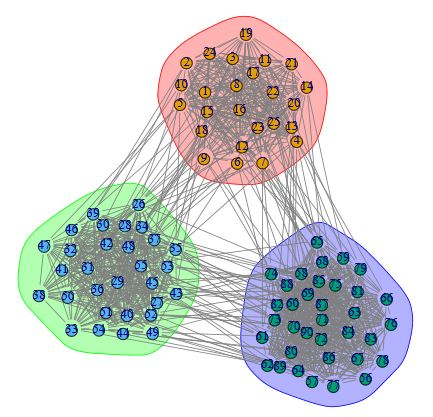
\includegraphics[scale=0.5]{SBM.JPG}
\caption[Visualization of an SBM-based graph example]{An example of a graph generated using SBM model, the graph has 90 nodes divided into three communities of size 25, 30 and 35 nodes. An edge between two nodes within the same community has a probability 0.8, while it has a probability 0.5 if the two nodes belong to different communities.}
%Source:
\label{fig:SBM_example}
\end{figure}

Note that the average degree $\mu_u$ of any node $u$ is given by:
\begin{equation}
    \mu_u=\Big[\sum_{b_i\neq b_u} p_{b_u,b_i}*(\#\{ u'\in \V, b_{u'}=b_i \} )\Big]+p_{b_u,b_u}*(\#\{u'\in \V, b_{u'}=b_u \}-1 )
\end{equation}

\subsection{Dataset setup}

In every experiment, unless otherwise mentioned, we generate a SBM dataset consisting of 300 graphs divided, 240 as a training set and 60 as a test set. Each graph has $v=60$ nodes divided equally between six communities $\eta=6$. Moreover, graphs are divided into two classes based on two different choices of the matrix $\mathbf{P}$. For the class $j\in\{0,1\}$, the matrix $\mathbf{P}_j$ contains $p_{in,j}$ on its diagonal as the intra-community edge probability and $p_{out,j}$ outside its diagonal.

%But the two matrices have something in common: $p_{1,1}= p_{2,2} = p_{in}$ and it is obvious that  $p_{1,2}=p_{2,1}=p_{out}$ too since we want an indirect graphs dataset as indicated previously.\newline
%Thus, the first class of graphs corresponds to a fixed pair ($p_{in,1}, p_{out,1}$) and similarly the second   corresponds to ($p_{in,2}, p_{out,2}$). \newline 
In order to prevent the two classes from being easily discriminated by the average degree of nodes in the graph as a feature, the two pairs of probabilities $(p_{in,j}, p_{out,j})$ are chosen such that all nodes have a fixed expected average degree equal to $\mu=10$. We denote by $r=(p_{in,1}/p_{in,0})$ the inter-classes similarity parameter: the closer $r$ is to $1$, the more similar both classes are, and thus the harder it is to discriminate them. We fix $p_{in,0} = 0.3$, and therefore the only parameter adjusted in the experiments is $r$.

\subsection{Histogram visualization}
Let us quickly visualize what are the histograms $\mathbf{f}_\G$ of graphlets that are manipulated by the classical graphlet kernel for our SBM data. We generate a graph $\G$ by SBM with a randomly chosen pair $(p_{in},p_{out})$, then we compare the following: exhaustive enumeration of all size-5 graphlets in $\G$, sampling $s=2000$ graphlets of the same size with uniform sampling, or sampling 2000 graphlets using random walks. For each case, we built using $\varphi^{match}_k$ a histogram of graphlets \emph{without repetition}. We show the three graphlet histograms in Fig. \ref{fig:graphlet_hist}. 

\begin{figure}[H]
\centering
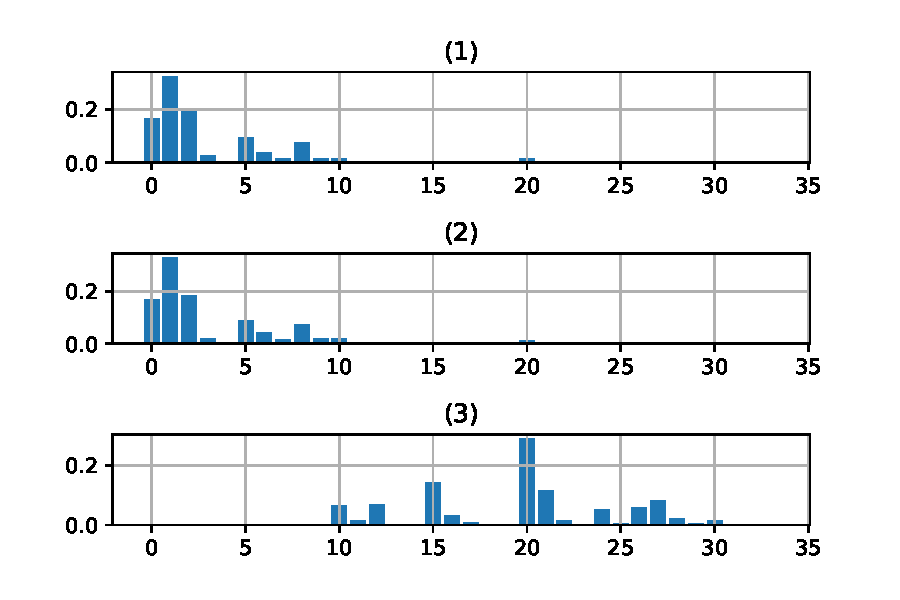
\includegraphics[scale=0.5]{class0_hist.pdf}
\caption[Graphlet histograms of uniform and random walk sampling techniques]{Size-5 graphlet histograms of an SBM random graph, with respecting the isomorphism test. (1): With exhaustive enumeration of all graphlets. (2): 2000 samples with uniform samples. (3): 2000 samples using random walks. }
%Source:
\label{fig:graphlet_hist}
\end{figure}

As expected, empirical uniform sampling provides a good approximation of exhaustive enumeration, and changing the sampling technique modify the histogram. Moreover, we ordered the graphlets such that the more disconnected graphlets are on the left and the connected graphlets on the right, and as expected random walk sampling tends to produce more connected graphlets than uniform sampling. In all the  following experiments we consider uniform sampling technique as our sampler and the adjacency matrix of a graphlet as an input, unless otherwise is mentioned.
\section{Choice of feature map $\varphi$}
In this section, we examine how the choice of $\varphi$ affects the performance and computation time of GSA-$\varphi$.
\begin{figure}[H]
\centering
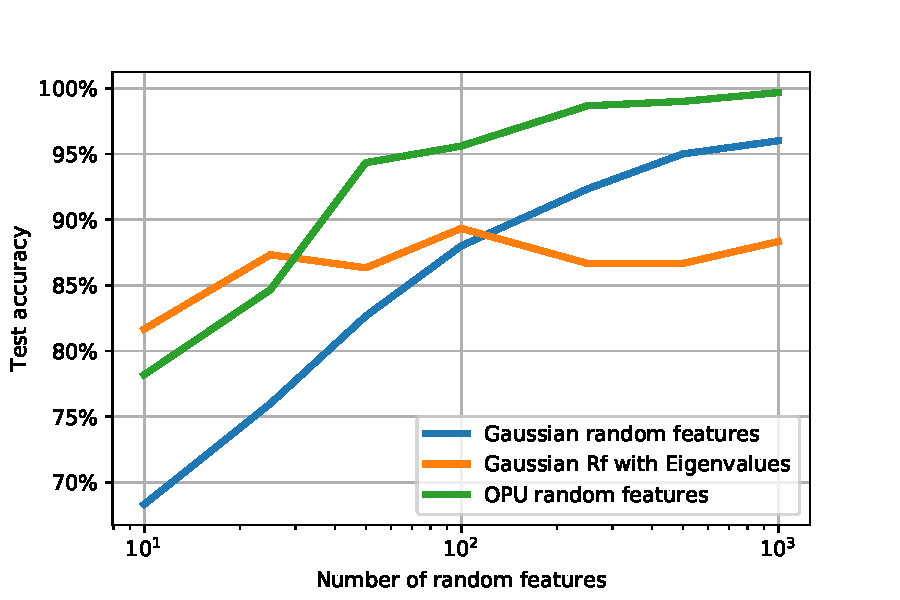
\includegraphics[scale=0.5]{figs/phi_comparison.pdf}
\caption[comparison between different choices of $\varphi$]{comparison between different choices of $\varphi$}
%Source:
\label{fig:phi_comparison}
\end{figure}

\begin{figure}[H]
\centering
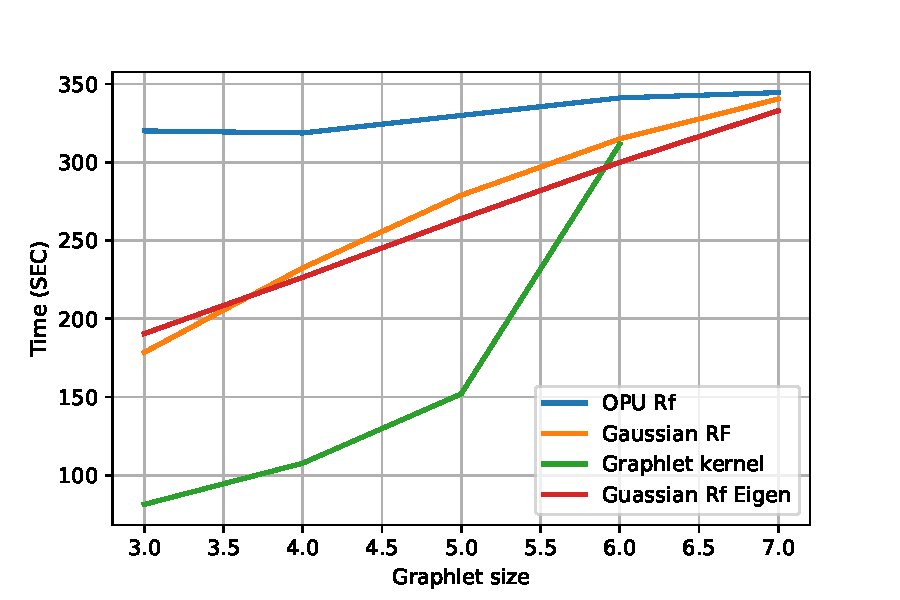
\includegraphics[scale=0.5]{figs/computational_comp.pdf}
\caption[Comparison in Computational cost between methods  ]{Comparison between different methods with respect to Computational cost  }
%Source:
\label{fig:computational_comparison}
\end{figure}



\section{Role of each parameter in $GSA-\varphi_{OPU}$}

In this section, we perform various experiments to examine the role of each parameter of GSA-$\varphi$ on the classification performance, using the optical random features $\varphi_{OPU}$.

\subsection{Number of samples $s$}
We first examine the minimum number of samples needed to classify both classes with high test accuracy (also called validation accuracy).

%\subsection{Varying the number of samples $s$}
We use the following parameters: number of random features $m=5000$, inter-class similarity $r=2$, and uniform sampling. These parameters were chosen such that the two classes can be efficiently classified with sufficiently large $s$ and large $k$. Then for three graphlet sizes $k\in\{4,5,6\}$, we vary the number of samples and plot the test accuracy in Fig. \ref{fig:varying_samples_num}.

 %To understand this we can consider the critical case when we use $k=1$ between two graphs, which means that we count how many nodes there are in each. Obviously this is a redundant choice since such graphlets don't provide a lot of information on how nodes are structured and connected in the graph. Thus, for each application, we must choose large $k$ so that graphlets include discriminative patterns not useless ones.
\begin{figure}[H]
\centering
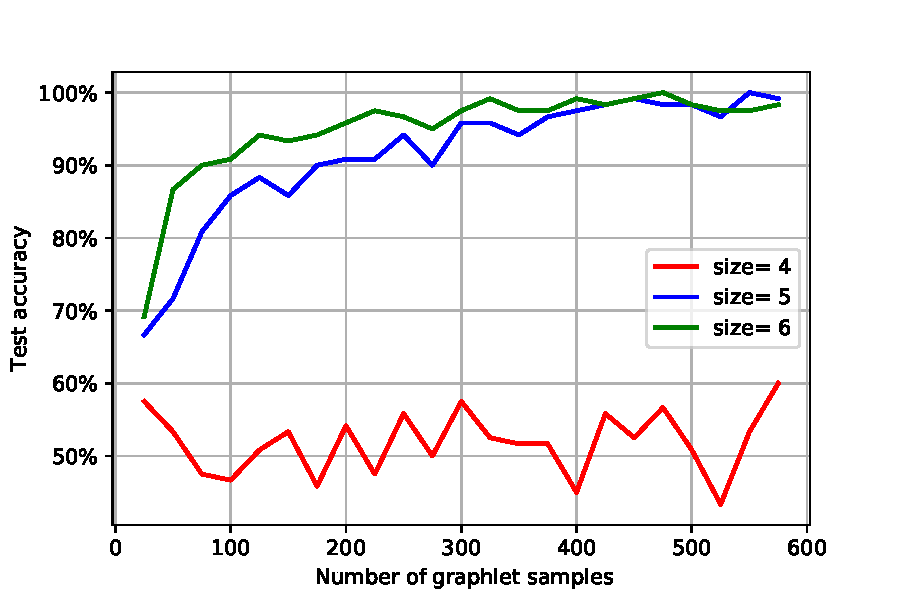
\includegraphics[scale=0.5]{samples_num.pdf}
\caption[$GSA-\varphi_{OPU}$ behavior with respect to number of samples $s$]{$GSA-\varphi_{OPU}$ behavior with respect to number of samples $s$. With $r=2,$, $m=5000$, $k\in\{4,5,6\}$, input: $\mathbf{A}$ and sampler: uniform sampling technique.}
%Source:
\label{fig:varying_samples_num}
\end{figure}
Results show that, in these settings, even with large number of samples the algorithm will not perform well if the graphlet size is too small. It is known that the algorithm is strictly more powerful for high graphlet size (for instance, $k=2$ only computes the density of edges), and it seems that here $k=4$ is unsufficient. %Secondly, %is that in this experiment and even in the next ones, we don't have access to apply the kernel which corresponds to OPUS' random features. That's why we cannot get sure that these results meets the concentration inequalities in chapter\ref{chapter:fast_algorithm}. 
However, we see that for $k\in\{5,6\}$, test accuracy increases as $s$ increases, and that a fairly low number of samples is enough to obtain good classification results. As shown in the previous sections, with higher number of samples the performance of the algorithm converges to the performance of the corresponding algorithm with exhaustive sampling.

\subsection{Number of random features $m$}
In this experiment we explore the role of random features number $m$ in our algorithm. 
Experiment setup: inter-class similarity: $r=1.1$, graphlet size: $k=6$, samples number $s=2000$, input: adjacency matrix $\mathbf{A}$, and uniform sampling.
In addition, for every value of $m$, we repeated the experiment $5$ times, and plot both individual results and average accuracies in Fig. \ref{fig:varying_random_features}. We can see that when $m$ grows, the average test accuracy gets higher, \emph{i.e.} we approximate the performance of the original mean kernel. Even further, as $m$ increases, the 5 experiments provide lower-variance accuracies, which is compatible with the concentration inequalities in chapter \ref{chapter:fast_algorithm}.

\begin{figure}[H]
\centering
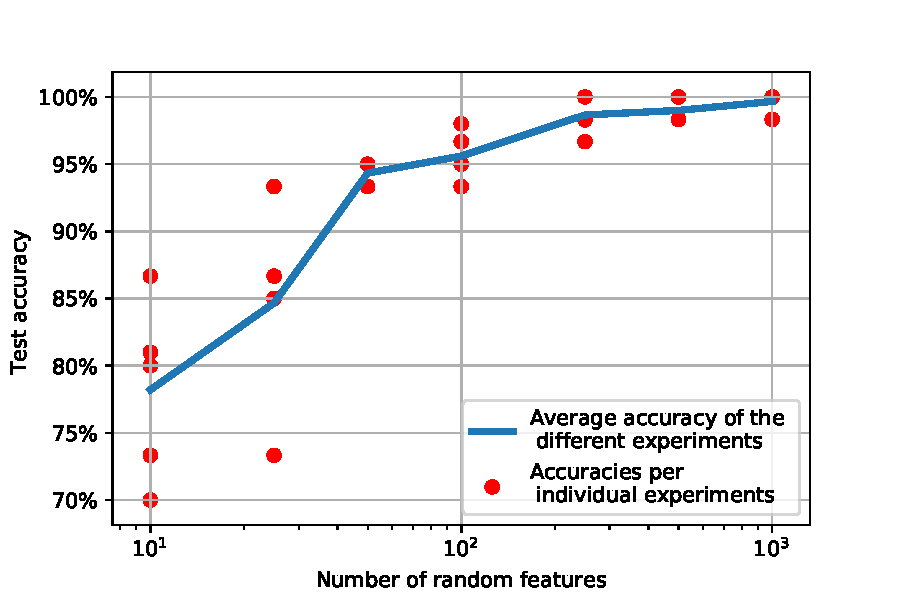
\includegraphics[scale=0.5]{LightON_adj_SBM_varying_RF.PDF}
\caption[$GSA-\varphi_{OPU}$ behavior with respect to number of random features $m$]{$GSA-\varphi_{OPU}$ behavior with respect to number of random features $s$. With  $r=1.1$, $k=6$, $m=5000$, input:$\mathbf{A}$ and sampler: uniform sampling technique. For every value of $m$, the experiment is done five times (red dots), then the $5$ resulted accuracies are averaged (blue curve).}
\label{fig:varying_random_features}
\end{figure}

\subsection{Sampling method}
Now we explore the role of the sampling technique in our algorithm. we do the experiment with the following parameters: samples number $s=2000$.
Then for three graphlet sizes $k\in\{3,4,5,6\}$, we vary the value of inter-classes similarity parameter $r$ and plot the test accuracy of both uniform and random walk sampling techniques, as shown in Fig. \ref{fig:comp_sampling}.
\begin{figure}
     \centering
     \begin{subfigure}[b]{0.4\textwidth}
         \centering
         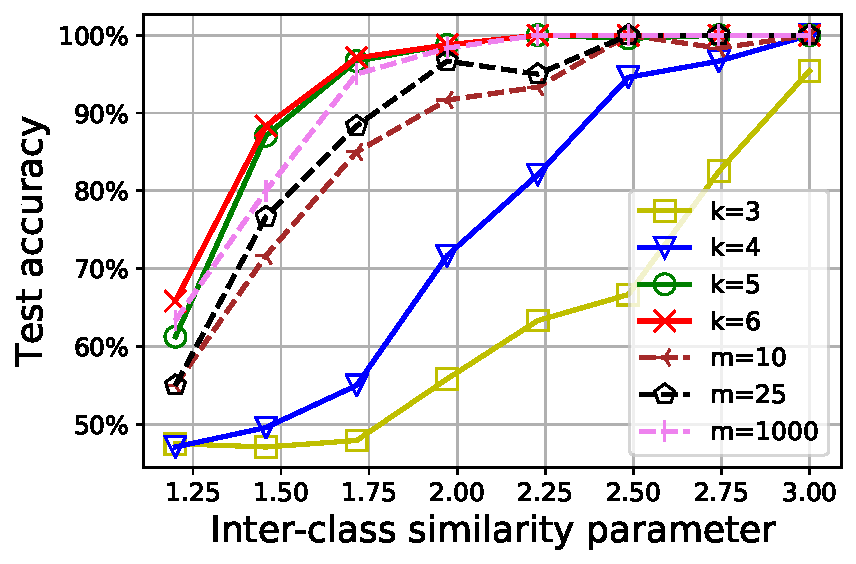
\includegraphics[width=\textwidth]{LightOn_adj_SBM_Similarity_graphlet_size.pdf}
         \caption{Uniform sampling}
         \label{fig:y equals x}
     \end{subfigure}
     \hfill
     \begin{subfigure}[b]{0.4\textwidth}
         \centering
         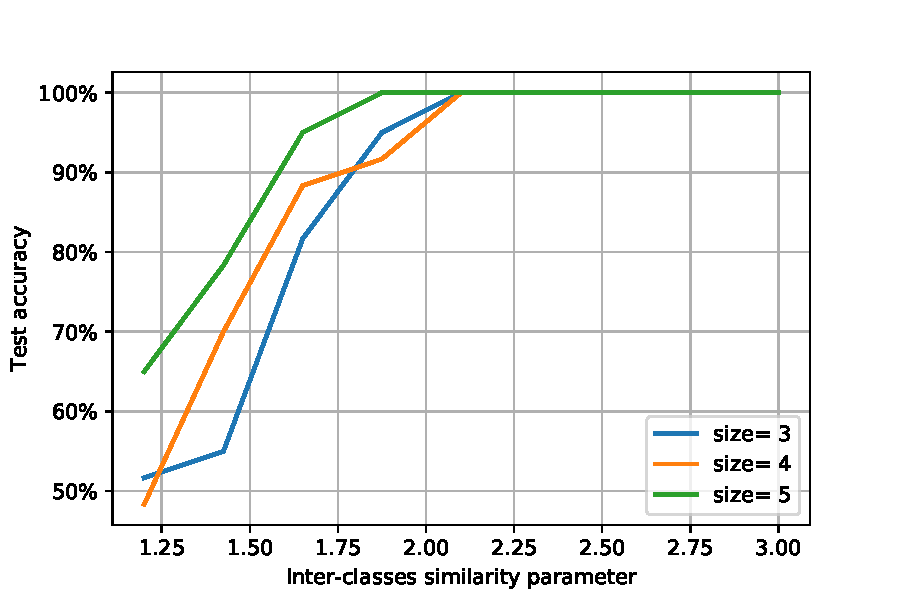
\includegraphics[width=\textwidth]{figs/LightOn_adj_SBM_similarity_graphlet_size_RW.pdf}
         \caption{Random walk sampling}
         \label{fig:three sin x}
     \end{subfigure}
        \caption [$GSA-\varphi_{OPU}$ behavior with respect to sampling technique]{$GSA-\varphi_{OPU}$ behavior with respect to sampling technique. With $m=5000$, $s=2000$, we vary the value of $r$ and plot the test accuracy of the algorithm when using uniform and random walk samplers. This is don for different graphlet sizes.}
%Source:
\label{fig:comp_sampling}
\end{figure}
Results show that for graphlet sizes $>5$, both sampling techniques perform similarly well. For uniform sampling, however, we notice that there is a gap between curves that correspond to $k=4$ and $k=5$, which is not noticed for the random walk sampler. This cannot be justified saying the size-4 graphlets are not informative, since random walk sampler performs well in that case. In fact, we don't have a justification for this phenomenon.  

\section{Comparison with graph convolution networks}
We modified and trained one of the proposed models built based on GIN (Graph Isomorphism Network). In graph classification, GIN model has been reported to give brilliant results, even better than most of state-of-the-art classical Graph convolutional networks \citep{GCN_powerful}. 
The model consists of 5 GIN layers followed by two fully connected layers where the dimensions of hidden layers are equal to 4. 

In this experiment, We trained then tested this model on our dataset with trying different values of inter-classes similarity parameter $r$, and results are shown in Fig. \ref{fig:GCN_GIN_SBM_multfactor_RW}
\begin{figure}[H]
\centering
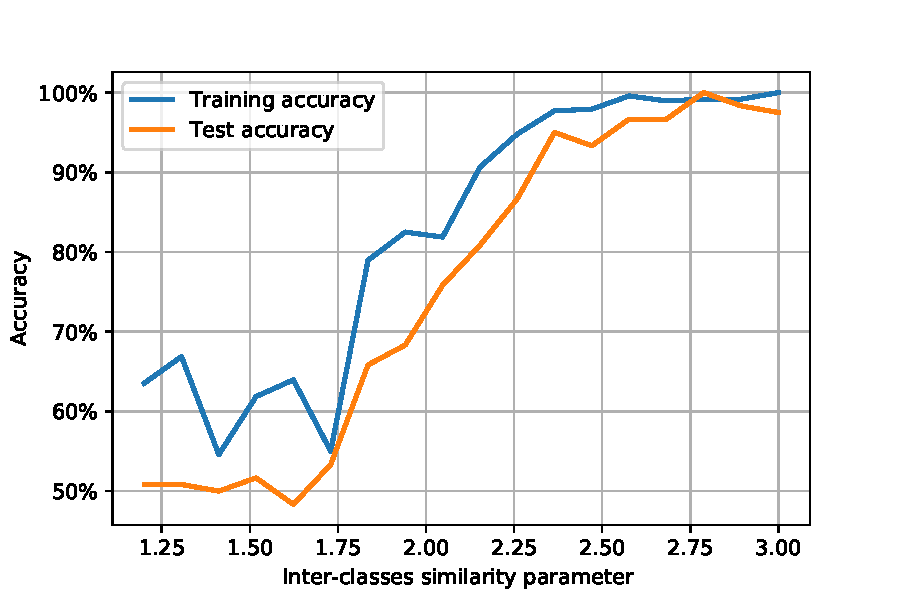
\includegraphics[scale=0.5]{GCN.pdf}
\caption[GCN model's classification test accuracy as a function of Inter-classes similarity parameter ]{GCN model's classification test accuracy with respect to Inter-classes similarity parameter. The  model is trained on SBM 240-sized labeled dataset.}
%Source:
\label{fig:GCN_GIN_SBM_multfactor_RW}
\end{figure}
Comparing GCN  to $GSA-\varphi_{OPU}$ (Fig. \ref{fig:comp_sampling}), we can see that $GSA-\varphi_{OPU}$ performs better when the graphlet size is greater than 4, especially using  random walk sampling technique. However, we didn't have access to high-speed graphical processing units (GPUs) to do the training process, thus we cannot compare both algorithms from computational-time point of view.

\section{Results on D\&D dataset}
D\&D is a dataset of size $n=1178$ graphs, each graph represents a protein structures \citep{DD_ref}. The nodes represent amino acids and two nodes are connected by an edge if they are less than 6 Angstroms apart. The problem  is to classify the protein structures into enzymes and non-enzymes. The extra thing here is that each node has 7 features, which is not used by our algorithms, \emph{i.e.} we will try to classify the graphs just based on their structure (topology).
We do the experiment with the following parameters inter-class similarity: graphlet size: $k=7$, samples number $s=4000$. 
In addition, for every value of $m$, we repeat the experiment $5$ times, and plot both individual results and average accuracies in Fig. \ref{fig:DD}. We can see that when $m$ grows, the average test accuracy gets higher, \emph{i.e.} we approximate the performance of the original mean kernel. Even further, as $m$ increases, the 5 experiments provide lower-variance accuracies, which is compatible with the concentration inequalities in chapter \ref{chapter:fast_algorithm}.

\begin{figure}[H]
\centering
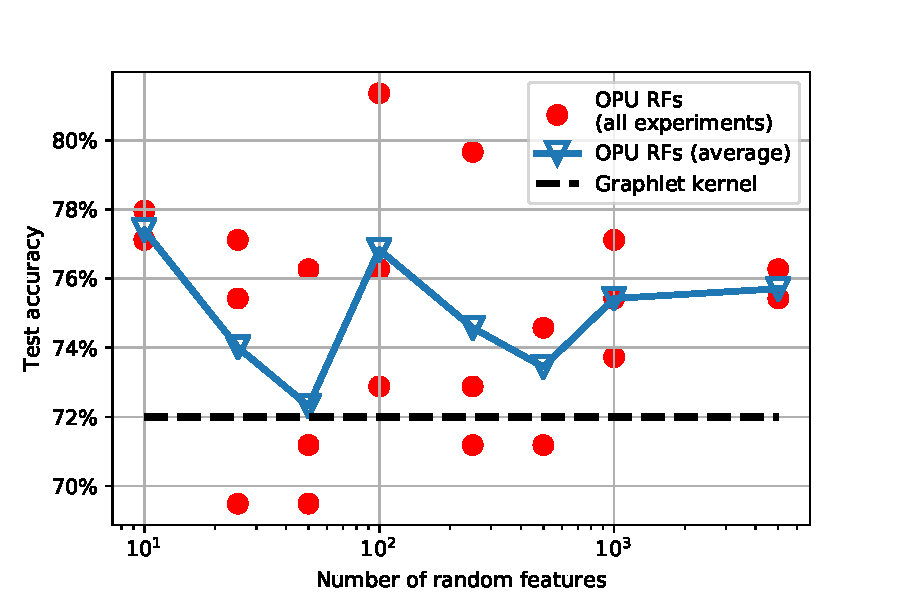
\includegraphics[scale=0.5]{DD.PDF}
\caption[$GSA-\varphi_{OPU}$ results on D\&D dataset]{$GSA-\varphi_{OPU}$ results on D\&D. With  $k=7$, $s=4000$. For every value of $m$, the experiment is done five times (red dots), then the $5$ resulted accuracies are averaged (blue curve).}
\label{fig:DD}
\end{figure}
The positive note here is that for when $m$ gets higher, the results of the 5 corresponding experiments get more concentrated around the average value. On the other hand, accuracy results show high variance with respect to $m$ itself if considered as a random variable. This is the result of ignoring the nodes features in each graph. However, it was interesting to touch the need to incorporate both sides of information.

\section{Conclusion and future work}
Graph kernels were for a long of time bunch of the efficient tools used in graph classification learning methods. However, many of them suffered from high computational time especially the well known \emph{graphlet kernel}. In this work, the task was to come up with a new algorithms that overcome this limitation. First, we did the necessary analysis on graphlet kernel. Then we studied how graph sampling is used to reasonably but not drastically accelerate the kernel. In fact, graphlet kernel with graph sampling inspired us to propose a new generic algorithm that put into use random features maps and graph sampling. More, importantly, defining the mean kernel in this algorithm, we could incorporate optical random features projections, which can be completed in light speed. After the full analysis done, we can surely say that our algorithm  both theoretically and empirically solved the computational time drawback. Furthermore, it preserved the efficiency of graphlet kernel and performed better than graph convolutional networks on graph classification.

\textbf{Future work:} One point left open to be analyzed is how to use our algorithm to classify graphs with node features. We saw previously that graph convolutional networks (GCN) has limits in learning just from the graph structure. So, one promising possibility is to use our algorithm to generate features embeddings on the graph level, and then feed these embeddings with the nodes' featureus of the graph to a deep neural network. By doing this, we take advantage of the speed of both our algorithm and GPUs. 



